% !TeX spellcheck = en_UK

\section{Calibration Methods in Radio Interferometry}\label{section.calibration}
\pg
In this section, we will discuss the implementation of interferometric array calibration. Our analysis is based on the RIME formalism, described in \cref{section.RIME}. One key metric of calibration quality is the \emph{dynamic range}, mentioned in Sec. \ref{section.clean}. High dynamic ranges mean that a high contrast has been obtained, and fainter sources can be reached. Here, because the difference between thermal noise and artefacts becomes relevant, we redefine dynamic range as follows
\begin{equation}\label{eq.DR}
DR = \frac{S_{max}}{S_{min},\max(\sigma_{thermal},\sigma_{artefacts})}
\end{equation}
where $S_{max}$ is the flux of the brightest source, $S_{min}$ the flux of the faintest source detectable above the noise, $\sigma_{thermal}$ the thermal noise in the image, and $\sigma_{artefacts}$ the noise associated with calibration artefacts. This gives a definition for dynamic range useful even in fields with a single source. We can thus use it as a metric for calibration quality specifically.

\pg
The distinction between these two noise sources is crucial; one can never go `below noise' for a given observation, no matter the quality of calibration. Astronomers typically observe for longer periods of time in order to reduce $\sigma_{thermal}$ in their images, but this will not reduce the artefacts caused by poor calibration solutions. Uncorrected Direction-Dependent Effects\footnote{See \cref{section.RIME.MultiplePointSources}} will not go away on their own, no matter how long the integration time. Similarly, there is a limit to how much improving calibration will improve the final image: eventually, more data is required to drive noise down.

\pg
We can distinguish three `generations' of calibration methods, of increasing complexity \citepads{2010A&A...524A..61N}. We will describe them in terms of the RIME, showing how each generation increases in generality to account for more exotic effects. They are referred to interchangeably as `nth-generation calibration' or `nGC' methods.

\subsection{Generational Analysis}

\subsubsection{First-Generation: Open-Loop Calibration}\label{section.calibration.1gc}

\pg
First-generation calibration methods (1GC methods) consist of open-loop calibration. This relies entirely on instrument stability, and thus imposes significant design constraints on radio telescopes. It consists of briefly observing an external calibrator before and after each observation run to find calibration solutions for those calibrator observations, and then interpolate between them over the ``target" observation. %\footnote{For a concrete example, see \href{http://www.analog.com/en/analog-dialogue/articles/open-loop-calibration-techniques.html}{the open-loop calibration techniques page of analog.com}.}
%\pg
%Phase calibration in the 1GC era `proper' was not necessary, as engineers were capable of ensuring adequate phase stability in contemporary interferometers. Phase was thus calculated relative to a fixed frame of reference, usually the central antenna of a 3-antenna array. 
In RIME terms (see \cref{section.RIME}), this consists of solving for a very basic form of $\Gjones_p$:
\begin{equation}
\Gjones_p = a_p \bm{\mathrm{I}} % \begin{bmatrix} e^{2 \pi i \nu ( \phi_p - \phi_0)} \end{bmatrix}
\end{equation}
where $a_p$ is a complex constant solved for during open-loop calibration. By interpolating between the two calibrator observations, it is possible to have a linear time-dependent gain estimate, though it is not much more complex than the above. %, $\nu$ the observing frequency, $\phi$ the phase at an antenna, and $\phi_0$ the phase at the reference antenna.

\pg
While values for $a_p$ and $b_p$ can in theory be found for both autocorrelation and both crosscorrelations (e.g. XY and YX for linear receptors), low signal-to-noise means that in practice, a single set of values is solved for per antenna\footnote{This reduces calibration to solving only for the intensity gains: the data can then only be used for \emph{intensity mapping} (e.g. \citepads{1957IAUS....4..159J}). This practice therefore precludes polarimetry.}. With these techniques, one can achieve dynamic ranges of about 100:1 (\citepads{2010A&A...524A..61N}).

\subsubsection{Second-Generation: Self-Calibration}\label{section.calibration.2gc}

\pg
Second-generation calibration methods (2GC methods) are defined by \emph{self-calibration}\footnote{On the discovery of self-calibration and its evolution in parallel to adaptive optics, see the chapter titled "The Almost Serendipitous Discovery of Self-Calibration'' in "\href{http://library.nrao.edu/public/collection/02000000000280.pdf}{\citep{serendipitous}}.}, commonly referred to as \emph{self-cal} (\citepads{1984ARA&A..22...97P}). As described in \cref{section.RIME.FullSky.CVZ}, this method can only be deployed if the brightness matrix of the sky is the same for all baselines\footnote{This is not to say that the brightness matrix must contain only point sources, but rather that moving our interferometer 500m to the East should not change its measured visibilities} (i.e. that we are not affected by direction-dependent effects).

\pg
The first instance of self-calibration (and adaptive optics in radio interferometry) is a paper published in the era of 1GC by Jennison \citepads{1958MNRAS.118..276J}, expanding on his PhD work, which was published in 1951). With sufficient signal-to-noise, he showed that \emph{phase closure} could be calculated and errors due to the atmosphere thus mitigated.

\pg
Self-calibration and adaptive optics are essentially the same thing, albeit meeting different constraints. Most notably, interferometric data is digital, allowing radio astronomers to perform their adaptive optics correction after the observation.

\pg
If amplitude and phase gains can be written as antenna-dependent, then each antenna-based error is estimated N times (once per each baseline which includes this antenna). By estimating, and correcting for, these errors, one can use a simple source model to infer an improved one. This is why the method is referred to as self-cal; by calibrating `on' a good calibrator source (bright, compact and unresolved), one can drastically improve one's source model, along with one's calibration solutions.


\begin{figure}[h!]
\centering
\resizebox{\hsize}{!}{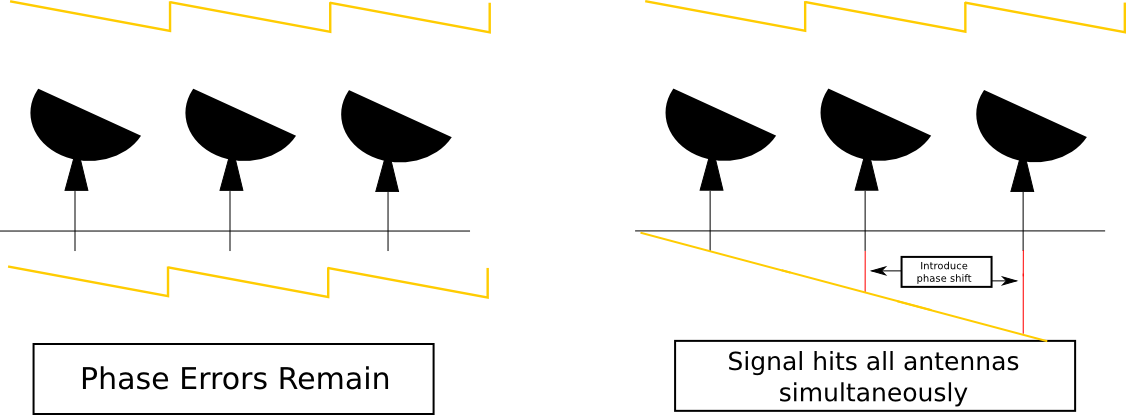
\includegraphics{images/selfcal.png}}
\caption{\label{fig.selfcal} Representation of self-calibration as adaptive optics}
\end{figure}

\pg
By extending this idea to VLBI (see e.g.  \citepads{1974ApJ...193..293R}), \emph{amplitude closure} was introduced to the field along with phase closure \citepads[as described in][]{1983Sci...219...51R}. These quantities are immune to antenna-based effects.%Astronomers were quick to apply these methods to interferometers in general.

\pg
The great advantage of radio interferometry over optics, however, is that we can \emph{iterate} over progressively improved source models. This is because interferometric data is digital, and because we record phase information.

\pg
In practice, of course, self-cal will be limited by noise. More precisely, it will be limited by sensitivity, in the form of the signal-to-noise ratio (henceforth SNR). For sufficiently bright sources, with high SNR, self-calibration can easily improve dynamic range by a factor of 10 (\cite{serendipitous}, p. 154) in a single iteration. 

\subsubsection{Third-Generation: Direction-Dependent Effects}

\pg
Third-generation calibration (3GC) is an extension of 2GC calibration which takes direction-dependent effects into account. At the time of writing, this is the cutting edge in radio interferometric calibration.

\pg
In this section, I will discuss the \emph{facet-based} approach taken by \citetads{2017arXiv171202078T}. The approach cannot be divorced from imaging, for the simple reason that solving for and applying Jones matrices\footnote{See \cref{section.RIME} for a full discussion on calibration and Jones matrices} in different directions requires image-plane knowledge of the sky brightness distribution $\Bmatrix$. % The imaging challenges this methods introduces will be discussed in [href to relevant imaging section].

\begin{figure}[ht]
\centering
\resizebox{\hsize}{!}{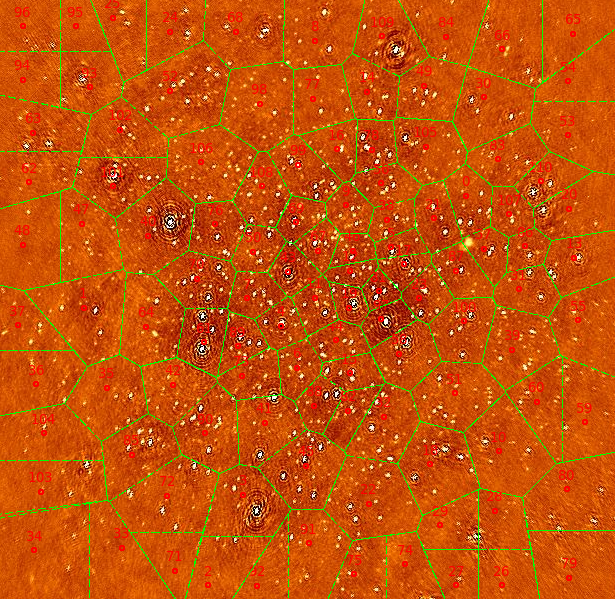
\includegraphics{images/bootes-image.png}}
\caption{\label{fig.facets} Voronoi facets, as implemented in DDFacet. Image is made before application of direction-dependent correction. This is an image of the Bootes field, made by Cyril Tasse.}
\end{figure}

\pg
When performing first and second-generation calibration, one solves for a set of Jones matrices or parameters thereof. Direction-independent calibration then consists of applying these calibration solutions to the visibilities directly. However, while these solutions will be correct in the direction of the calibrator source, they are increasingly likely to be wrong as a function of distance from said calibrator source. The difference between the true gains in a given direction and the gains estimated from the calibrator source are called \emph{differential gains}.

\pg
Why then not solve for a set of calibration solutions for each source in the calibration model, iteratively adding new sources to this model as they become above the noise as calibration artefacts - introduced by poor calibration - decrease? There are two main reasons for this: firstly, the SNR when calibrating using very faint source models will be poor. This means that gains will likely be extremely noisy, and applying them will result in increased calibration artefacts in the final image. Secondly, even by optimising for signal-to-noise and only using a few of the brightest sources in the field, the problem quickly becomes intractably large in terms of computing power required, provided that standard complex differentiation is used \citepads[see][]{2016ApJS..223....2V}. Wirtinger differentiation \citepads[see][]{2014arXiv1410.8706T,2015MNRAS.449.2668S} does alleviate this somewhat by allowing the Hessian matrix to be written as a block-diagonal matrix, but is not implemented in all standard direction-dependent calibration software at the time of writing.

\pg
The crucial insight of a faceting approach is then to split the image into a set of \emph{facets}, solving for a set of calibration solutions for each of these facets. These solutions are then applied to the visibilities when mapping them onto the dirty image. The faceting in DDF is shown in \cref{fig.facets}. The facet distribution shown in \cref{fig.facets} encourages an even flux distribution in multiple facets, and ensures that no facet is so small that too little signal would be available within. As we can see from \cref{fig.DDcal.effect}, direction-dependent calibration can drastically improve the quality of wide-field images. It currently represents the state of the art in interferometric calibration. 

\begin{figure}[h!]
\centering
\begin{subfigure}{\textwidth}
\resizebox{\hsize}{!}{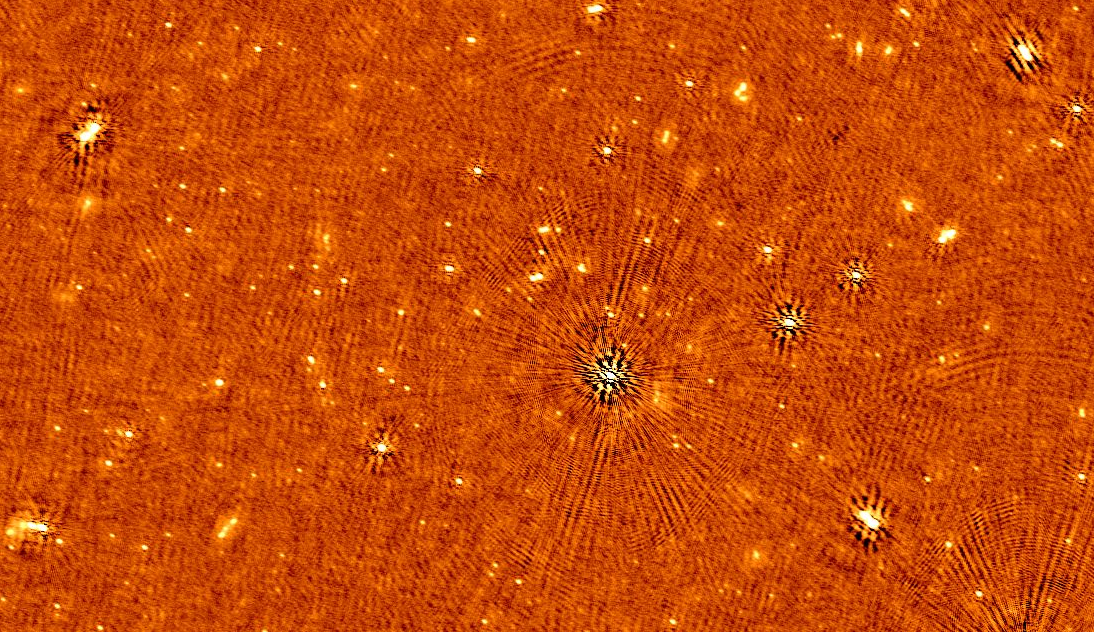
\includegraphics{images/lofar-nocorr.png}}
\caption{\label{fig.lofar.noDDcal} Image of the Boötes field, made without direction-dependent calibration. Image by Cyril Tasse.}
\end{subfigure}
\begin{subfigure}{\textwidth}
\resizebox{\hsize}{!}{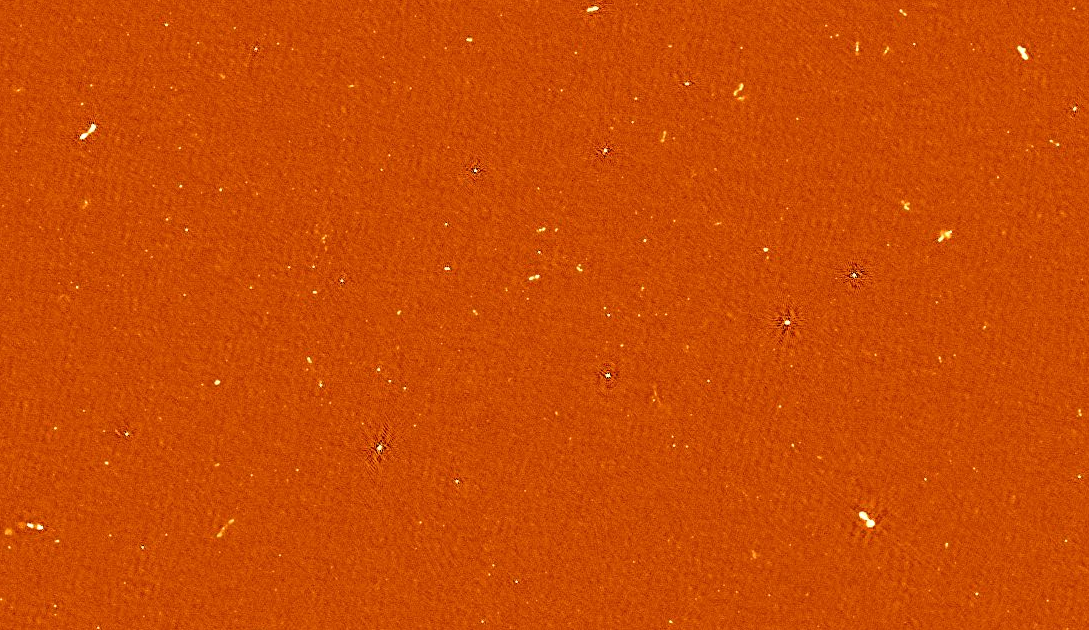
\includegraphics{images/lofar-corr.png}}
\caption{\label{fig.lofar.withDDcal} Image of the same Boötes field, made with direction-dependent calibration. Image by Cyril Tasse.}
\end{subfigure}
%\hfill
\caption{\label{fig.DDcal.effect} Difference between imaging made with (Fig. \ref{fig.lofar.withDDcal})and without (Fig. \ref{fig.lofar.noDDcal}) third-generation calibration.}
\end{figure}







